\textbf{如下图所示,发送窗口与发送缓存以及接收窗口与接收缓存有什么区别?为什么计算机进行通信时发送缓存和接收缓存总是需要的?}

\textbf{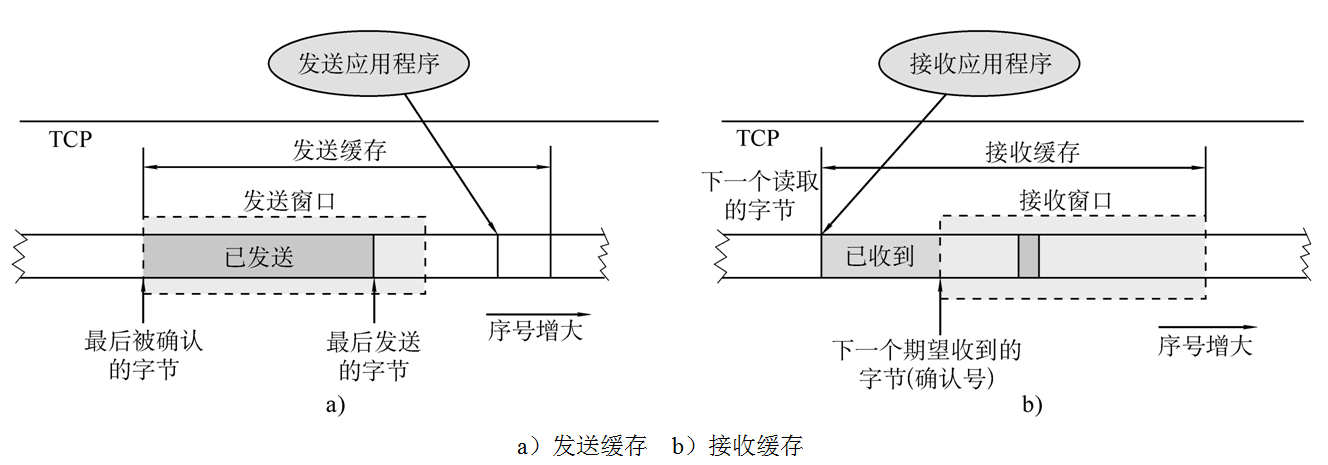
\includegraphics[width=3.33333in,height=1.16667in]{png-jpeg-pics/47491CE31EE01CEECE0A88EF4E528713.png}\\
}

从上图b)中可以看到,按序到达的且没有被交付给主机的帧被放在\textbf{接收缓存}(接收窗口外的那一部分接收缓存,以下讲的接收缓存都是指这部分)里面(因为已经发送过确认帧了,仅仅是等主机的应用程序来取),而不是接收窗口里面。那些不是按序到达的数据且没有错误的帧一定是要放在接收窗口里面,因为这些帧不能直接给主机,而放在\textbf{接收缓存}的帧是要给主机的,等到缺少的帧收到后,再一起放到接收缓存,这一点要注意区分,其他都比较好理解,不再赘述。

\textbf{发送窗口的大小不一定等于接收窗口的大小(但是通常情况下都是等于),这里先记住这个结论,第5章讲到拥塞控制的时候就会很清楚了。}

当计算机的两个进程(在同一台机器中或在两个不同的机器中)进行通信时,如果发送进程将数据直接发送给接收进程,那么这两个动作(一个是发送,另一个是接收)是非常难协调的。这是因为计算机的动作很快,如果在某一时刻接收进程开始执行接收的动作,但发送进程的发送动作稍微早了一点或稍微晚了一点(在收发双方事先未进行同步的情况下,发送时刻不可能恰好和接收时刻精确地重合),这都会使接收失败。

\textbf{综上所述,}在计算机进程之间的通信过程中,广泛使用{缓存}。缓存就是在计算机的存储器中设置的一个临时存放数据的空间。

\textbf{发送进程将欲发送的数据先写入缓存},然后接收进程在合适的时机读出这些数据。{缓存}类似于邮局在街上设立的邮筒。人们可以将欲发送的信件投到邮筒中。邮局的邮递员按照他的计划在适当的时候打开邮筒,将信件取走,交到邮局,进行下一步处理。缓存可以很好地解决发送速率和接收速率不一致的矛盾,还可以很方便地进行串并转换,即比特流串行写入并行读出,或并行写入串行读出。\textbf{缓存也可称为缓冲或缓冲区}(有关缓存更详细的讲解可参考《操作系统高分笔记》)。
